\begin{pastexam}[label={px:df3-101-ds-02}]{地方三等資訊處理 101 年 第二題}
（申論；20 分）

有個二元搜尋樹（binary search tree），若用後序瀏覽（postorder traversal）每個點得到的順序為：
\{20, 25, 15, 45, 36, 65, 75, 95, 90, 100, 86, 55\}。
\begin{itemize}[leftmargin=2.2em]
\item[㈠] 請畫出這個二元搜尋樹。（10 分）
\item[㈡] 請寫出用前序瀏覽（preorder traversal）每個點所產生的順序。（5 分）
\item[㈢] 用您建立的二元搜尋樹來搜尋 75，需要做幾次的比較（comparison）並寫出過程？（5 分）
\end{itemize}
\end{pastexam}

\begin{pastsoln}
答案：㈠ 樹如下圖；㈡ 55, 36, 15, 25, 20, 45, 86, 75, 65, 100, 90, 95；㈢ 比較 $3$ 次（55、86、75）。

\textbf{㈠} 二元搜尋樹的中序就是由小到大，所以等於知道了中序和後序，可以用重建的方法（資結書第~7.4~節）；
更簡單的是直接用二元搜尋樹的性質切：後序的最後一個是根，其餘的數裡比根小的是左子樹、比根大的是右子樹，
而且在後序裡左子樹的全部排在右子樹前面。
\begin{center}
\small
\begin{tabular}{lll}
\toprule
後序 & 根 & 左子樹 ／ 右子樹（後序） \\
\midrule
20, 25, 15, 45, 36, 65, 75, 95, 90, 100, 86, 55 & 55 & 20, 25, 15, 45, 36 ／ 65, 75, 95, 90, 100, 86 \\
20, 25, 15, 45, 36 & 36 & 20, 25, 15 ／ 45 \\
20, 25, 15 & 15 & 空 ／ 20, 25 \\
20, 25 & 25 & 20 ／ 空 \\
65, 75, 95, 90, 100, 86 & 86 & 65, 75 ／ 95, 90, 100 \\
65, 75 & 75 & 65 ／ 空 \\
95, 90, 100 & 100 & 95, 90 ／ 空 \\
95, 90 & 90 & 空 ／ 95 \\
\bottomrule
\end{tabular}
\end{center}
每一列的「比根小的」都正好是前面連續一段、「比根大的」是後面一段，所以這個後序確實是某棵二元搜尋樹的後序，
而且樹是唯一的。
\begin{center}
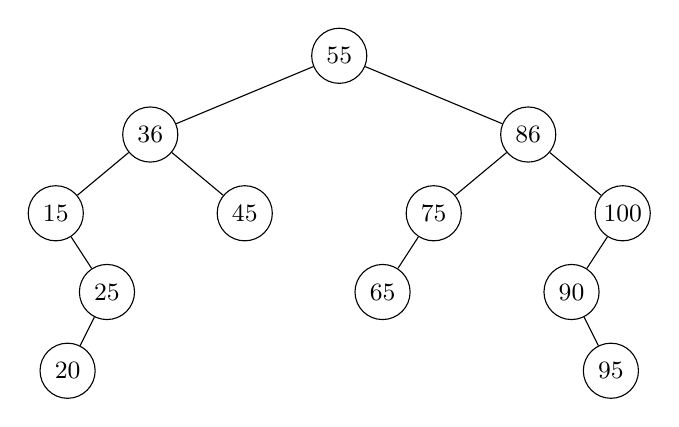
\begin{tikzpicture}[v/.style={circle,draw,minimum size=7mm,inner sep=0pt,font=\small},
    level distance=10mm, level 1/.style={sibling distance=48mm},
    level 2/.style={sibling distance=24mm}, level 3/.style={sibling distance=13mm},
    level 4/.style={sibling distance=10mm}]
\node[v] {55}
  child {node[v] {36}
    child {node[v] {15} child[missing] {} child {node[v] {25} child {node[v] {20}} child[missing] {}}}
    child {node[v] {45}}}
  child {node[v] {86}
    child {node[v] {75} child {node[v] {65}} child[missing] {}}
    child {node[v] {100} child {node[v] {90} child[missing] {} child {node[v] {95}}} child[missing] {}}};
\end{tikzpicture}
\end{center}
檢查：這棵樹的中序是 15, 20, 25, 36, 45, 55, 65, 75, 86, 90, 95, 100（由小到大），後序和題目一樣。

\textbf{㈡} 前序（根、左、右）：55；左子樹 36, 15, 25, 20, 45；右子樹 86, 75, 65, 100, 90, 95。 合起來：
\[
55,\ 36,\ 15,\ 25,\ 20,\ 45,\ 86,\ 75,\ 65,\ 100,\ 90,\ 95.
\]

\textbf{㈢} 從根開始，每到一個節點拿 $75$ 和它的鍵比較（資結書第~9.1~節）：
\begin{enumerate}[label=(\arabic*)]
\item 和根 $55$ 比較：$75 > 55$，往右子樹走。
\item 和 $86$ 比較：$75 < 86$，往左子樹走。
\item 和 $75$ 比較：相等，找到。
\end{enumerate}
共比較 $\mathbf{3}$ 次（$75$ 在第 $3$ 層，深度 $2$，比較次數 $=$ 深度 $+ 1$）。 若把「$<$、$=$、$>$」各算
一次比較（每個節點先比相等、再比大小），前兩個節點各 $2$ 次、最後一個 $1$ 次，共 $5$ 次；一般作答以每個
節點算一次，答 $3$ 次。
\end{pastsoln}
